\graphicspath{{\relativepath/figures/}}

\subsection{Components of the simulator}

The simulator can be decomposed into several large modules that handle specific tasks during simulation (Fig. \ref{presentation}). First of all, there is an \textbf{input/output} module that creates everything that is needed for the simulation from an input file (Fig.~\ref{presentation} - Initialization). \textbf{Reactants} and \textbf{reactions} are user-specified and need to be created on demand, as well as \textbf{events} happening throughout the simulations and more technical aspects about which algorithm to use to perform the integration. Once everything is set up, the \textbf{solver} follows a simple loop that can be decomposed in three steps (Fig.~\ref{presentation} - Loop). Integration occurs reaction by reaction, at each loop, we go forward one reaction, update the simulation time, concentrations and reaction rates.

\begin{enumerate}
	\item At the beginning of the loop, the \textbf{input/output} process checks whether \textbf{events} should occur at the current simulation time and whether it needs to write some concentrations to an output file.
	\item It then hands control over to the \textbf{solver}, which is based on Gillespie's approach to integrate a network of chemical reactions. The Gillespie algorithm needs the current reaction rates of all \textbf{reactions} and draws a random reaction with a probability proportional to its rate. This task is delegated to a \textbf{rate manager}, which uses state-of-the-art methods to maintain the rate list updated and perform the drawing efficiently.
	\item Once a \textbf{reaction} is drawn, it is performed \textit{i.e.} the concentrations (and the state, see below) of its \textbf{reactants} is modified.
\end{enumerate}

\begin{figure}[!ht]
	\centering
	\includegraphics[width=0.8\linewidth]{presentation}
	\caption{Schematical view of the simulator.}
	\label{presentation}
\end{figure}


\subsection{Reactant hierarchy}

This section gives a quick overview of the contents of the \textbf{reactant} module. More details about how reactants are implemented can be found later.

\subsubsection{UML class diagram}

\begin{figure}[!ht]
	\centering
	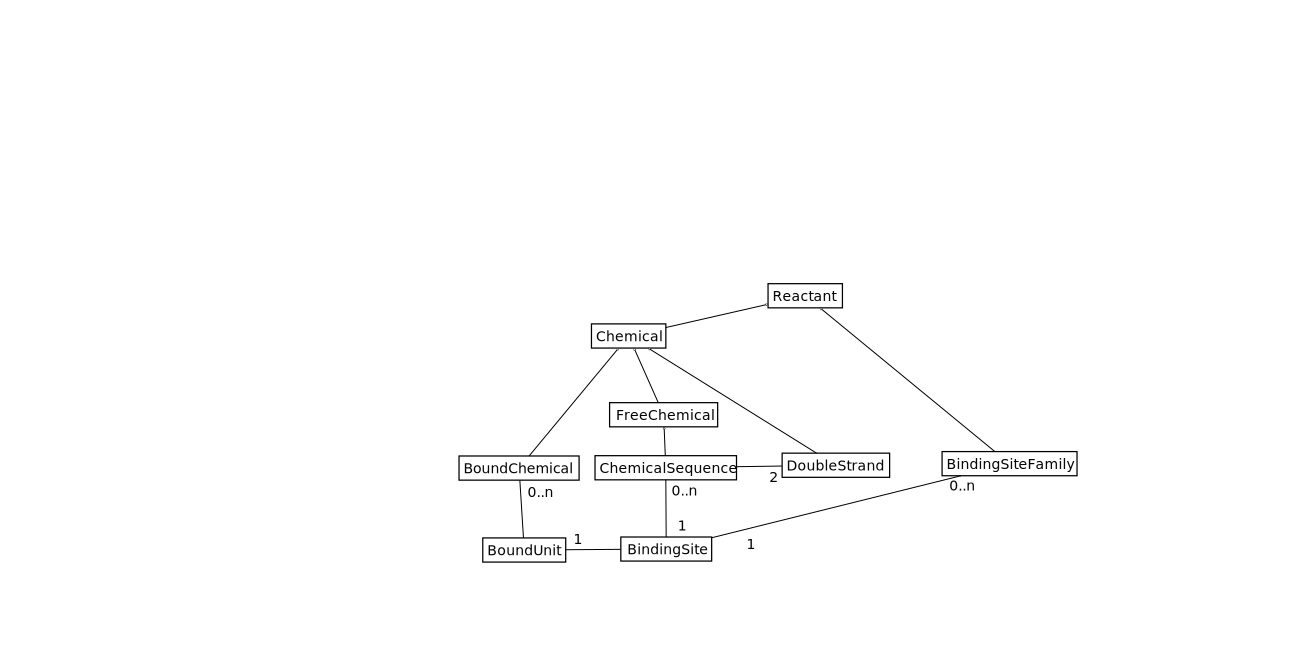
\includegraphics[width=0.8\linewidth]{reactant_uml}
\end{figure}

\subsubsection{Reactant}

\texttt{Reactant} is a global abstract interface. All entities that can participate in a reaction \emph{must} inherit from it.

\subsubsection{Chemical}

\begin{figure}[!ht]
	\centering
	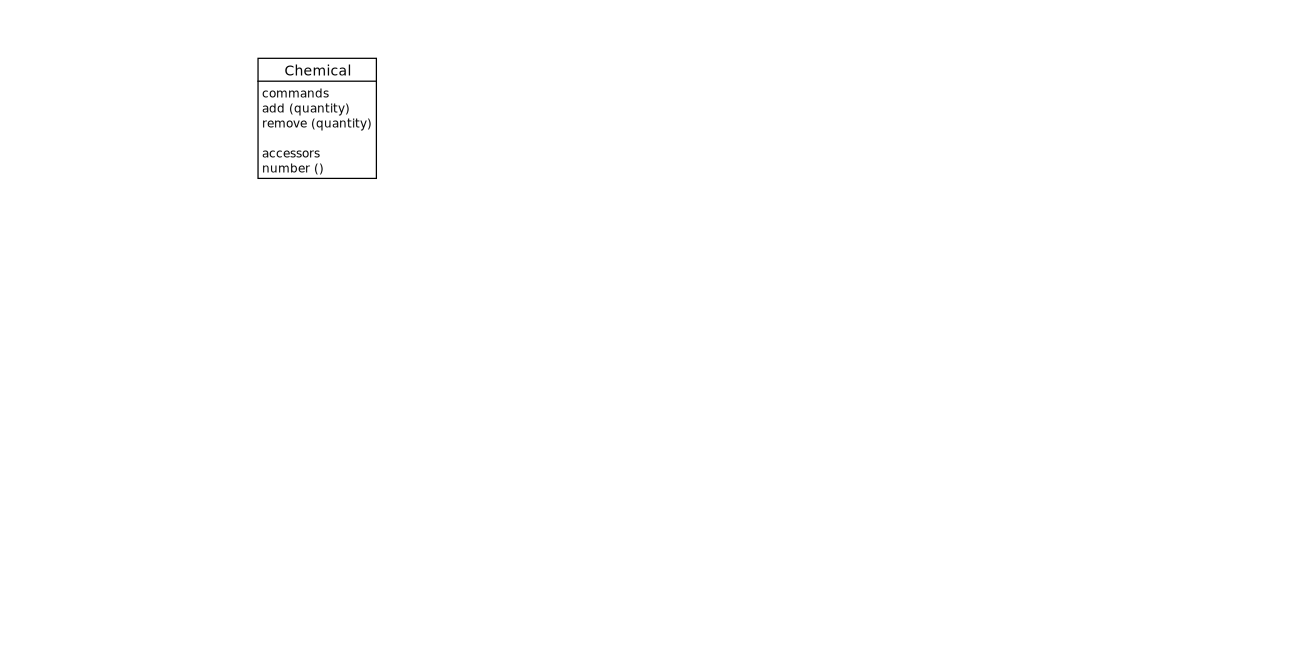
\includegraphics[scale=0.8]{chemical}
\end{figure}

\texttt{Chemical} is an abstract class. It defines all standard chemical entities. \texttt{Chemical} represents a \emph{pool} of a given chemical species, meaning that one may access its current number at any time.

\subsubsection{FreeChemical}

\paragraph{Input format}
\begin{verbatim}
FreeChemical <name> [<initial quantity>]
\end{verbatim}

\begin{figure}[!ht]
	\centering
	\includegraphics[scale=0.8]{freechemical}
\end{figure}

\texttt{FreeChemical} is a subclass of \texttt{Chemical} that represents free chemical (\textit{e.g.} molecules diffusing in the cytosol or extracellular medium).

\subsubsection{BoundChemical}

\paragraph{Input format}
\begin{verbatim}
BoundChemical <name>
\end{verbatim}

\begin{figure}[!ht]
	\centering
	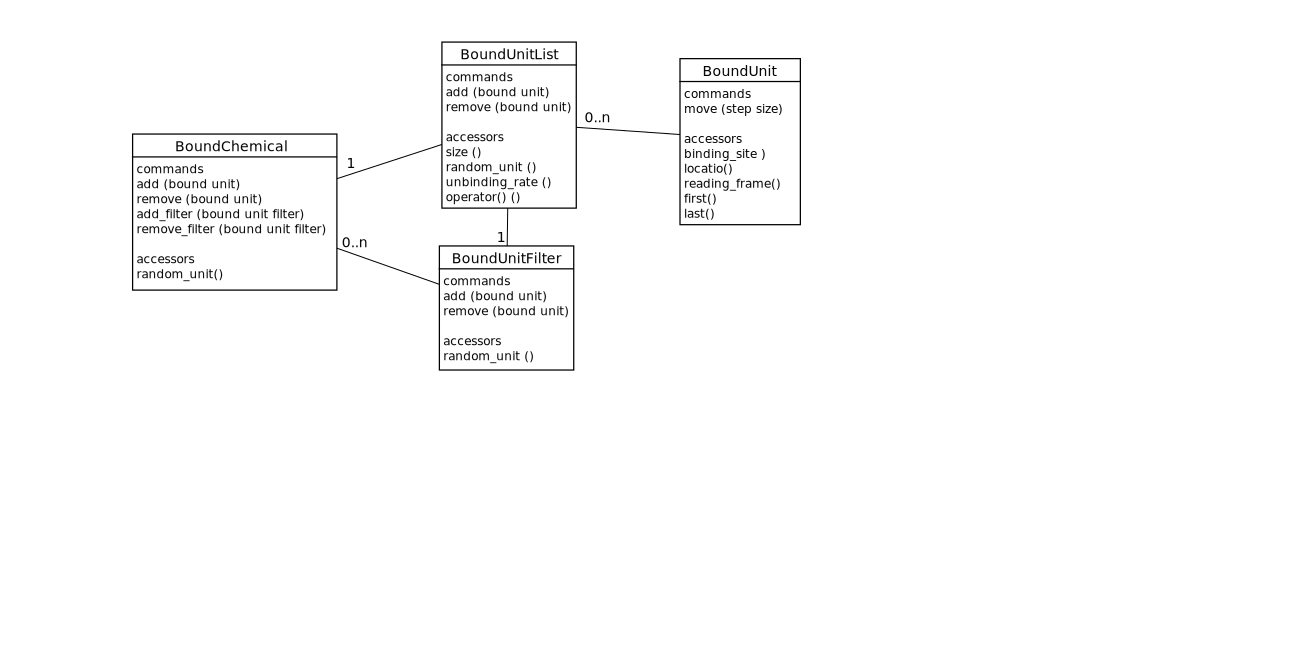
\includegraphics[scale=0.8]{boundchemical}
\end{figure}

\texttt{BoundChemical} is a subclass of \texttt{Chemical} that represents chemicals that are bound to a sequence. It is important to note it only represents molecules bound to the sequence, \emph{not} the complex formed by the chemical and the sequence. Even though \texttt{BoundChemical} represents a pool of molecules, single elements are not interchangeable, they are defined by their position on a sequence. \texttt{BoundChemical} uses two classes \texttt{BoundUnit} and \texttt{BoundUnitList} to represent molecules individually. It uses \texttt{BoundUnitFilter} to organize bound units according to outside criteria needed for reactions (classify according to binding sites, templates read, etc.).

\subsubsection{ChemicalSequence}

\paragraph{Input format}
\begin{verbatim}
ChemicalSequence <name> sequence <sequence> [<initial quantity>]
TransformationTable <name> [<parent_letter> <product_letter>,]^{1..n}
ProductTable <name> <transformation table>
ChemicalSequence <name> product_of <parent sequence> \
  <starting position> <ending position> <product table> [<initial quantity>]
\end{verbatim}

\begin{figure}[!ht]
	\centering
	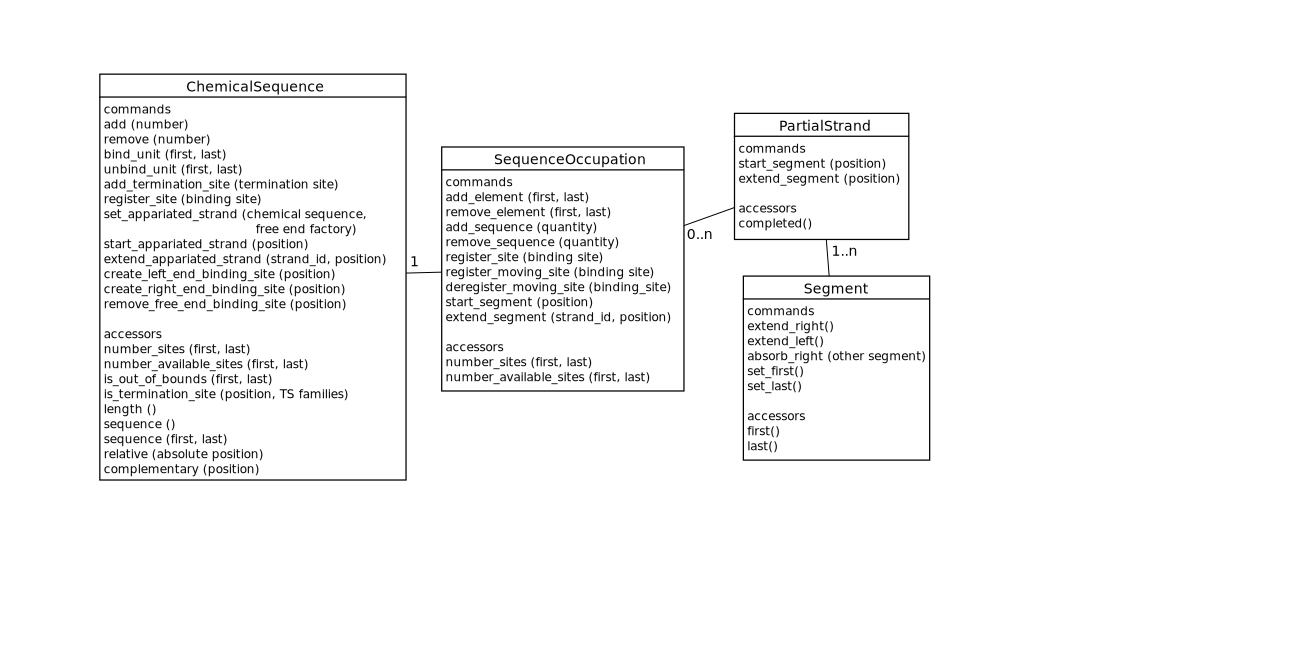
\includegraphics[scale=0.7]{chemicalsequence}
\end{figure}

\texttt{ChemicalSequence} is a subclass of \texttt{FreeChemical}. It is defined by a sequence and the ability to bind elements. However, instances of a sequence are \emph{not} treated individually, it is impossible to tell to which instance a given chemical bound. An object called \texttt{SequenceOccupation} maintains occupation levels at sites of interest. For example, suppose the sequence is an mRNA carrying a ribosome binding site for the protein DnaA. The number of available sites is obtained by removing the number of bound chemicals occupying the site from the number of instances of the mRNA currently in the cell. A \texttt{ChemicalSequence} can be appariated to another \texttt{ChemicalSequence}. New instances can be created segment wise, which is handled by classes \texttt{PartialStrand} and \texttt{Segment}. A \texttt{ChemicalSequence} can be created from a sequence or as a product of another sequence, in which case a \texttt{TransformationTable} is needed to generate the product's sequence from the parent's, and a \texttt{ProductTable} stores the parent/product relationship.

\subsubsection{DoubleStrand}

\paragraph{Input format}
\begin{verbatim}
TransformationTable <name> [<letter> <complementary_letter>,]^{1..n}
DoubleStrandSequence <name> <name_sense_sequence> <sense_sequence> \
  <name_antisense_sequence> <transformation_table> [<initial quantity>]
\end{verbatim}

\begin{figure}[!ht]
	\centering
	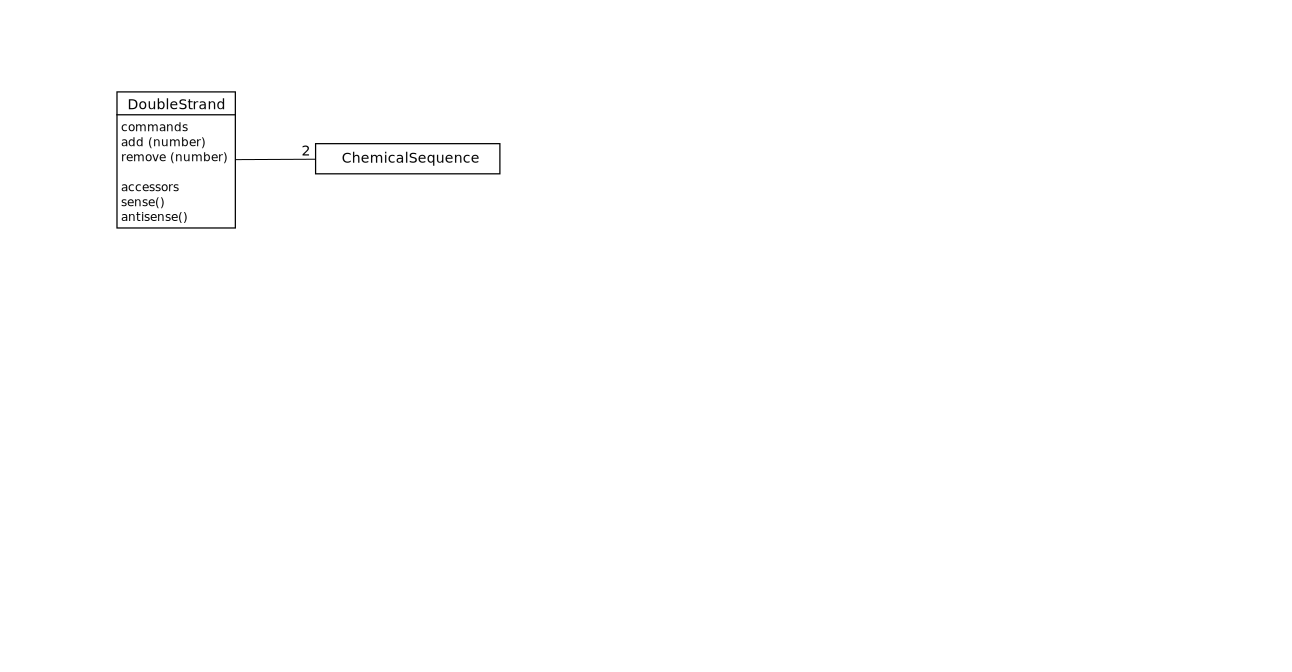
\includegraphics[scale=0.8]{doublestrand}
\end{figure}

\texttt{DoubleStrand} links two \texttt{ChemicalSequence} together that are biochemically linked (\textit{e.g.} DNA), one sequence being complementary to the other. It enables segment extension on the appariated strand and free end binding (see interface of \texttt{ChemicalSequence}). A \texttt{DoubleStrand} is created from a sense sequence that is specified similarly to a \texttt{ChemicalSequence}. However, the complementary sequence is created from a \texttt{TransformationTable} that specifies how to transform the sense sequence into antisense sequence (\textit{e.g.} for DNA, $A\rightarrow T$, $T\rightarrow A$, $C\rightarrow G$, $G\rightarrow C$).

\subsubsection{BindingSiteFamily}

\begin{figure}[!ht]
	\centering
	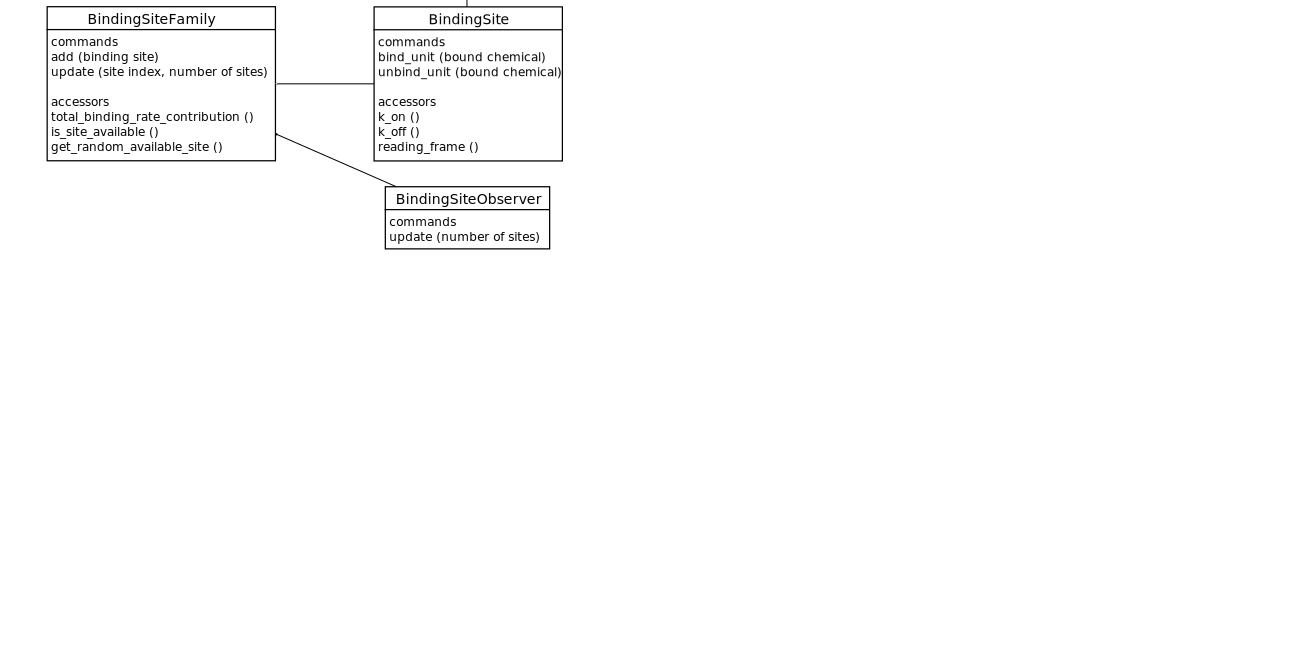
\includegraphics[scale=0.8]{bindingsitefamily}
\end{figure}

\texttt{BindingSiteFamily} is a subclass of \texttt{Reactant}. Contrary to \texttt{Chemical}, it does not represent a countable pool of molecules. Each family contains a number of related instances of \texttt{BindingSite} (\textit{e.g.} ribosome binding sites). \texttt{BindingSiteFamily}, \texttt{BindingSite} and \texttt{ChemicalSequence} use a notification pattern (via \texttt{update} methods) to dynamically maintain the number of available sites for each binding site as well as binding rates up to date. If a binding site is used to load polymerases, a reading frame should be provided to specify where a polymerase will start reading the sequence after binding.

\paragraph{Input format}
\begin{verbatim}
BindingSite <binding site family name> <chemical sequence> \
  <start> <end> <k_on> <k_off> [<reading frame>]
\end{verbatim}



\subsection{Reaction hierarchy}

This section gives a quick overview of the reaction module. More details about how reactions are implemented can be found later.

\subsubsection{UML class diagram}

\begin{figure}[!ht]
	\centering
	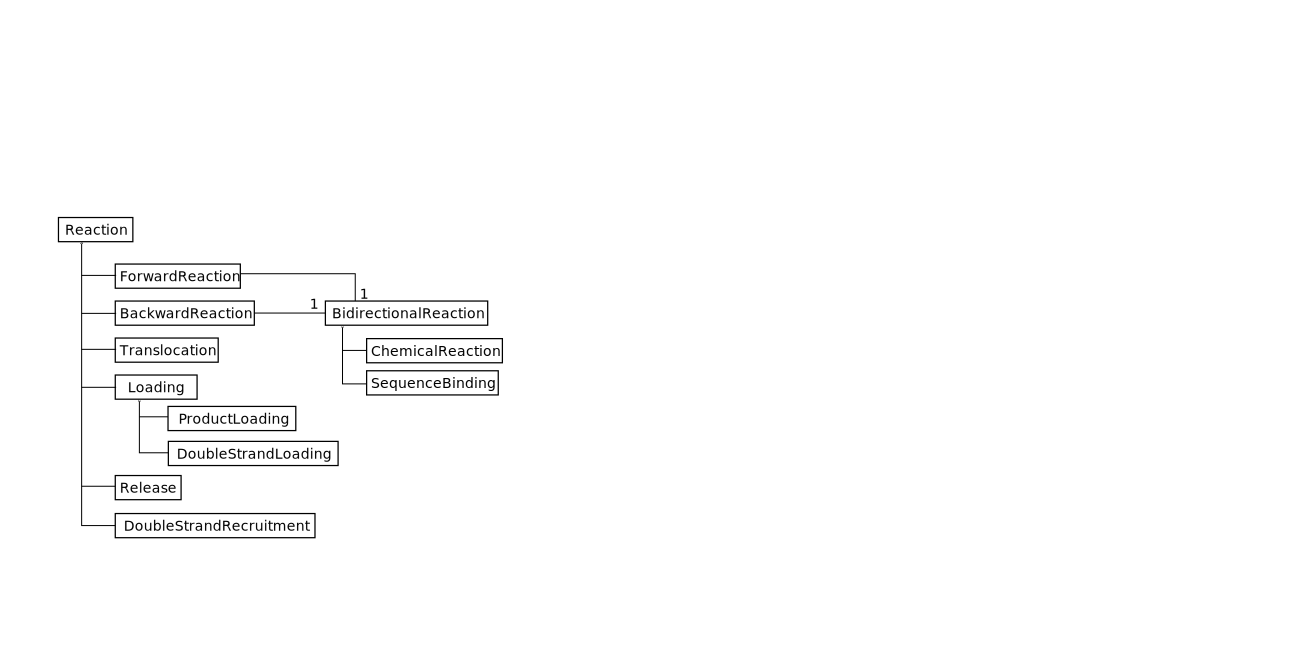
\includegraphics[width=0.8\linewidth]{reaction_uml}
\end{figure}

\subsubsection{Reaction}

\begin{figure}[!ht]
	\centering
	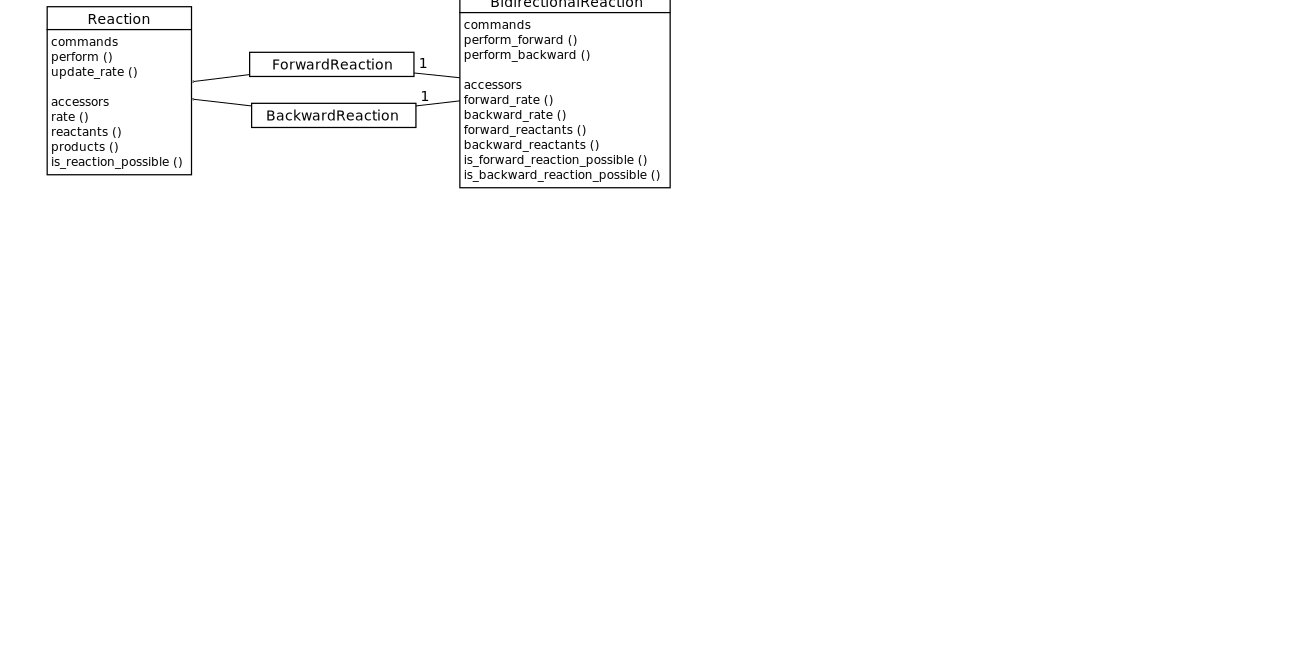
\includegraphics[width=0.8\linewidth]{reaction}
\end{figure}

There are two abstract classes used to define reactions: \texttt{Reaction} for one-way reactions and \texttt{BidirectionalReaction} for reversible reactions. Two adapter classes \texttt{ForwardReaction} and \texttt{BackwardReaction} split reversible reactions in two one-way reactions. In the end, the solver only handles one-way reactions. A reaction can necessarily be performed, its rate updated and accessed and is composed of reactants and products.

\subsubsection{ChemicalReaction}

\begin{figure}[!ht]
	\centering
	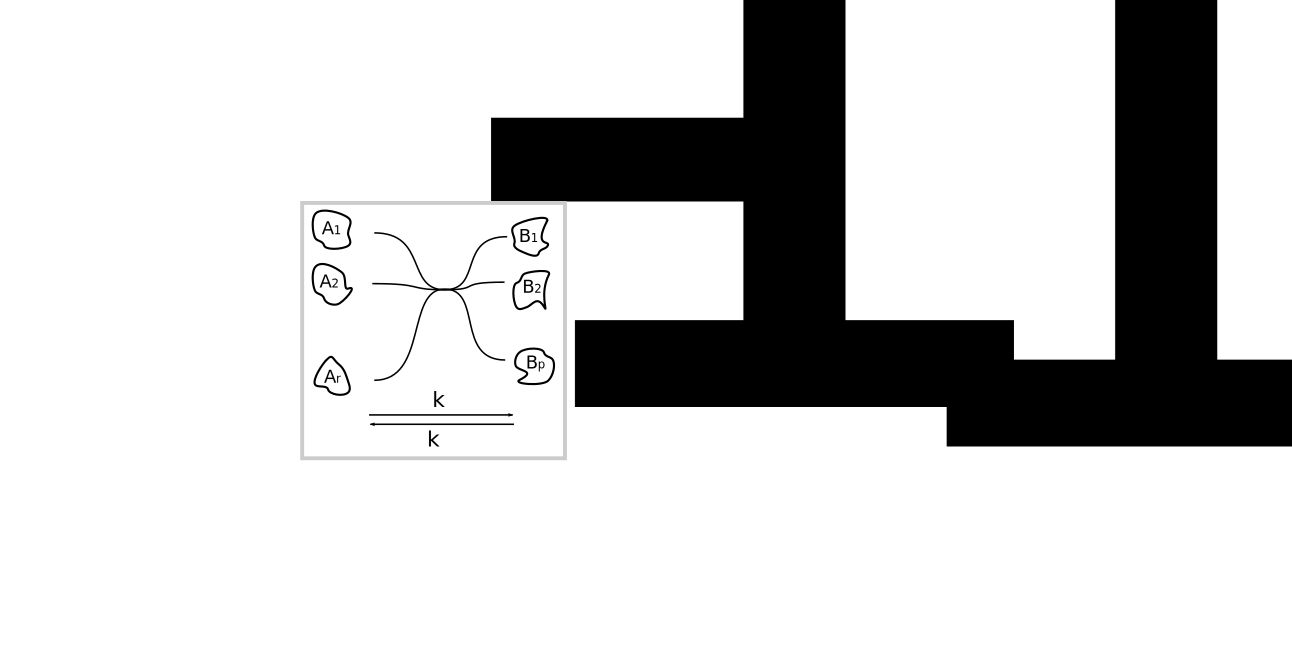
\includegraphics[scale=0.8]{chemicalreaction}
\end{figure}

\paragraph{Input format}
\begin{verbatim}
ChemicalReaction [<chemical> <stoichiometry>]^{1..n} rates <k_1> <k_-1>
\end{verbatim}

\paragraph{Formula} A \texttt{ChemicalReaction} represents association/dissociation of an arbitrary number of elements. It is defined by
$$
	\reactionRev{a_1 A_1 + a_2 A_2 + ... + a_r A_r}{b_1 B_1 + ... + b_p B_p}{k_1}{k_{-1}}
$$
where
\begin{itemize}
	\item $A_i$ and $B_i$ are of type \texttt{FreeChemical}. They can be of type \texttt{BoundChemical}, \emph{if} there is exactly one \texttt{BoundChemical} on each side of the equation and the associated stoichiometric coefficient is 1. 
	\item $a_i$ and $b_i$ are stoichiometric coefficients.
	\item $k_1$ and $k_{-1}$ are rate constants.
\end{itemize}

\paragraph{Action} When the reaction is performed, the number of chemicals involved is changed according to their stoichiometric coefficient. If \texttt{BoundChemical} are involved, the simulator will assume that the bound chemical that is consumed is replaced by the bound chemical on the other side of the equation (\textit{i.e.} it will be bound at the location previously occupied by the precursor).

\paragraph{Rate} The rates are given by
$$
	\lambda_{forward} = k_1 \prod\limits_{i=1}^{r} [A_i]^{a_i}
$$
$$
	\lambda_{backward} = k_{-1} \prod\limits_{i=1}^{p} [B_i]^{b_i}
$$

\subsubsection{SequenceBinding}
\paragraph{Input format}

\begin{figure}[!ht]
	\centering
	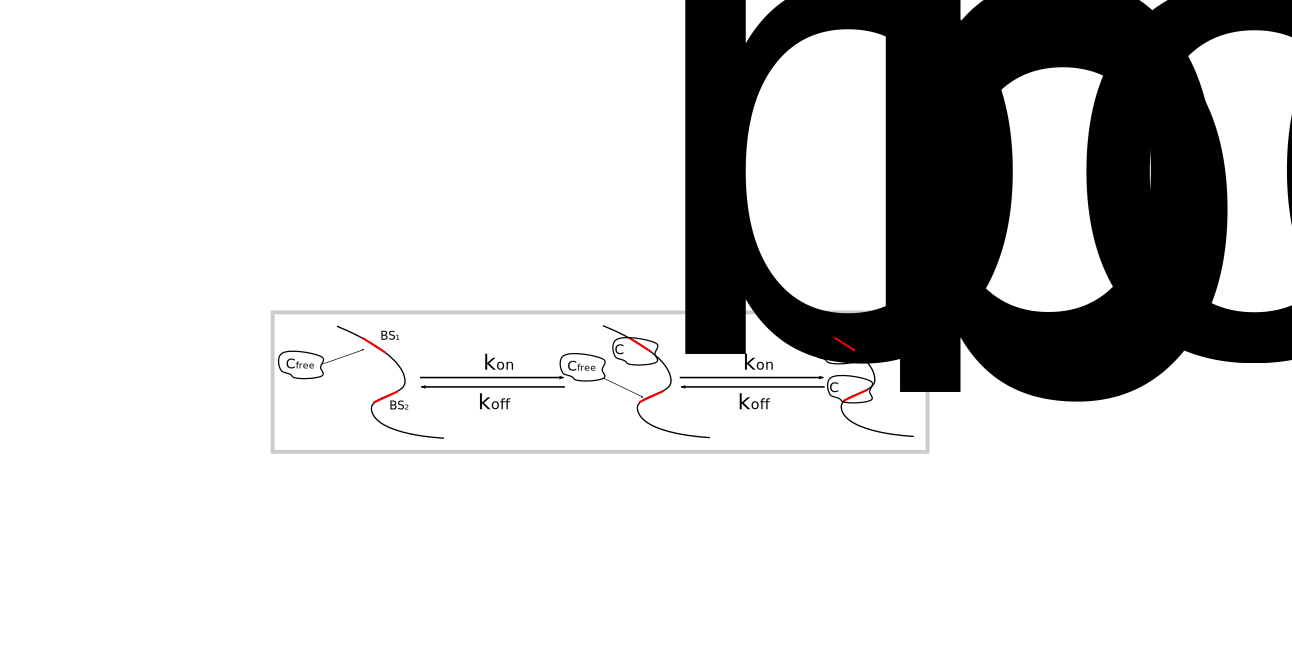
\includegraphics[scale=0.8]{sequencebinding}
\end{figure}

\begin{verbatim}
SequenceBinding <chemical> <bound form> <binding site family>
\end{verbatim}

\paragraph{Formula} A \texttt{SequenceBinding} represents binding of a free element on a binding site of a sequence. It is defined by
$$
	\reactionRev{C_{free} + BSF}{C_{bound}}{}{}
$$
where
\begin{itemize}
	\item $C_{free}$ is of type \texttt{FreeChemical}.
	\item $BSF$ is of type \texttt{BindingSiteFamily}.
	\item $C_{bound}$ is of type \texttt{BoundChemical}.
\end{itemize}

\paragraph{Action} When the forward reaction is performed, a random available binding site is drawn from the binding site family (drawing is weighted by affinity). A $C_{free}$ molecule is removed from the pool and a $C_{bound}$ added to the \texttt{ChemicalSequence} bearing the binding site. When the backward reaction is performed, a random molecule of $C_{bound}$ is removed from the pool (and from its sequence) and a $C_{free}$ molecule is added.

\paragraph{Rate} The rates are given by
$$
	\lambda_{forward} = \frac{[C_{free}]}{V_c} \sum_{\text{sites }s \in BSF} (k_{on})_s \times \text{Number of sites $s$ available}
$$ 
$$
	\lambda_{backward} = \frac{1}{V_c} \sum_{\text{molecules }m \in C_{bound}} (k_{off})_\text{site on which $m$ is bound}
$$
\begin{itemize}
	\item $(k_{on})_s$ is the association constant of $C_{free}$ with binding site $s$.
	\item $(k_{off})_s$ is the dissociation constant of $C_{bound}$ with binding site $s$.
	\item $V_c$ is the volume of the cell.
\end{itemize}

\subsubsection{Translocation}

\begin{figure}[!ht]
	\centering
	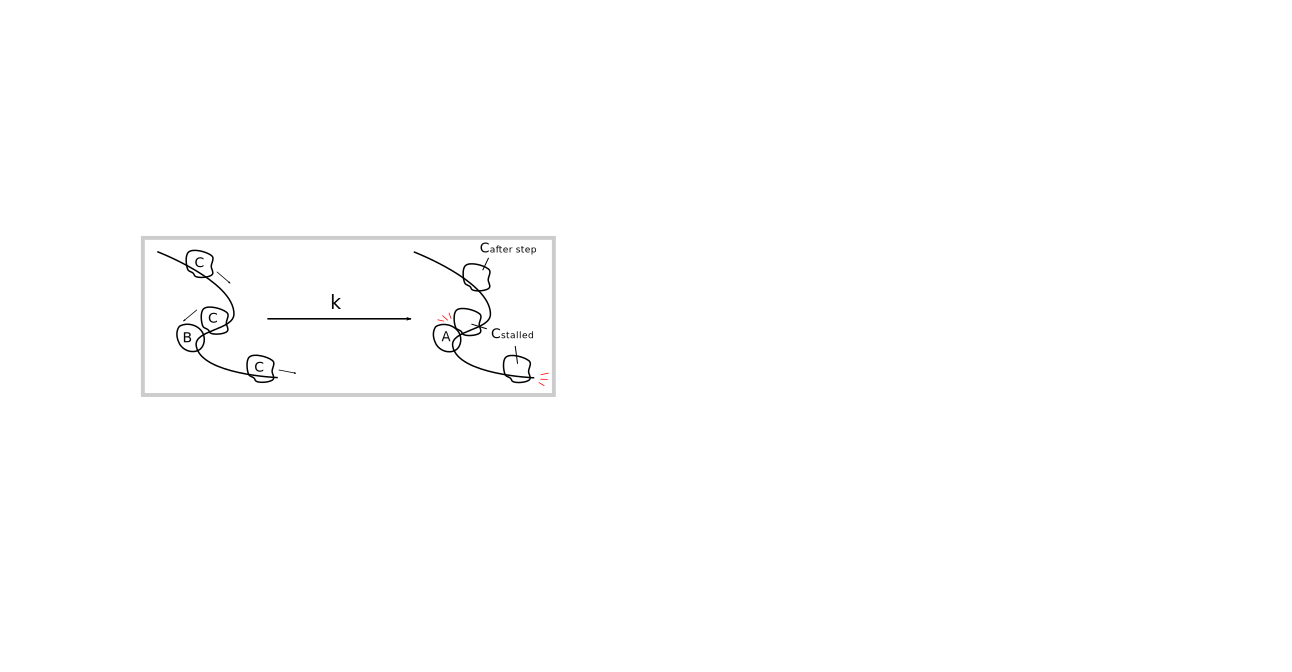
\includegraphics[scale=0.8]{translocation}
\end{figure}

\paragraph{Input format}
\begin{verbatim}
TerminationSite <family name> <chemical sequence> <start> <end>
Translocation <bound chemical> <form after step> <stalled form> \
  <step size> <rate> [<termination site family>]^{0..n}
\end{verbatim}

\paragraph{Formula} A \texttt{Translocation} represents movement of a bound element along a sequence. It is defined by
$$
	\reactionIrr{C}{C_\text{after step}}{k}{}
$$
or
$$
	\reactionIrr{C}{C_\text{stalled form}}{k}{}
$$
where
\begin{itemize}
	\item $C$ is of type \texttt{BoundChemical}.
	\item $C_\text{after step}$ is of type \texttt{BoundChemical}.
	\item $C_\text{stalled form}$ is of type \texttt{BoundChemical}.
	\item $k$ is a rate constant.
\end{itemize}

\paragraph{Action} When the reaction is performed, a random $C$ is chosen. Generally, it is replaced by a $C_\text{after step}$, moved by a step of a given size along the sequence the original $C$ is bound to. If the chemical cannot move because it reached the end of the sequence or it reaches a termination site, it is replaced by $C_\text{stalled form}$.

\paragraph{Rate} The rate is given by
$$
	\lambda = k [C]
$$

\subsubsection{Loading}

\begin{figure}[!ht]
	\centering
	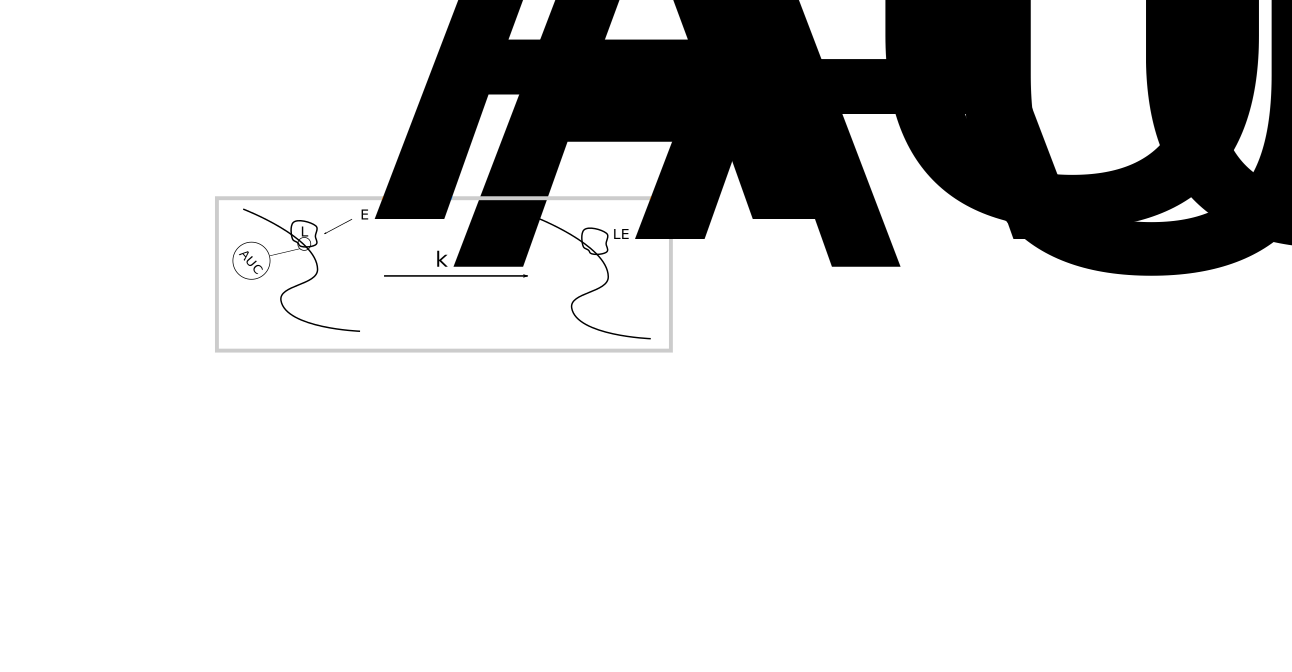
\includegraphics[scale=0.8]{loading}
\end{figure}

\paragraph{Input format}
\begin{verbatim}
LoadingTable <name> [<template> <element_to_load> <occupied_polymerase>,]^{1..n}
ProductLoading <bound chemical> <loading table>
DoubleStrandLoading <bound chemical> <loading table> <stalled form>
\end{verbatim}

\paragraph{Formula} A \texttt{Loading} typically represents loading of elements by a polymerase onto a template sequence. It is defined by
$$
	\reactionIrr{L + E}{LE}{}{}
$$
where
\begin{itemize}
	\item $L$ is of type \texttt{BoundChemical}.
	\item $E$ is an element to load, of type \texttt{FreeChemical}. It is defined in a \texttt{LoadingTable} associated with the reaction.
	\item $LE$ is the occupied form of the loader, of type \texttt{BoundChemical}. It is defined in a \texttt{LoadingTable} associated with the reaction.
\end{itemize}

\paragraph{Action} Each instance of $L$ reads a specific template. Using its \texttt{LoadingTable}, we know which $E$ it tries to load, which $LE$ is yielded if loading occurs and the loading rate associated with the template. When the reaction is performed, a random $L$ is chosen according to loading rates. An element to load $E$ is removed from the pool and $L$ is replaced with $LE$. A \texttt{ProductLoading} assembles loaded elements into a product that will eventually be release in the cytosol (\textit{e.g.} RNA synthesis), while \texttt{DoubleStrandLoading} extends segments along a \texttt{DoubleStrand} (\textit{e.g.} DNA replication). In \texttt{DoubleStrandLoading}, loading may fail because the loader met a previously synthesized segment. In the latter case, it is replaced by a \texttt{BoundChemical} representing its stalled form.

\paragraph{Rate} The rate is given by
$$
	\lambda = \sum_{t\in templates} k_t[L_t][E_t]
$$
where
\begin{itemize}
	\item $k_t$ is the loading rate associated with template $t$.
	\item $L_t$ corresponds to loaders $L$ reading template $t$.
	\item $E_t$ is the chemical to load onto template $t$.
\end{itemize}

\subsubsection{Release}

\begin{figure}[!ht]
	\centering
	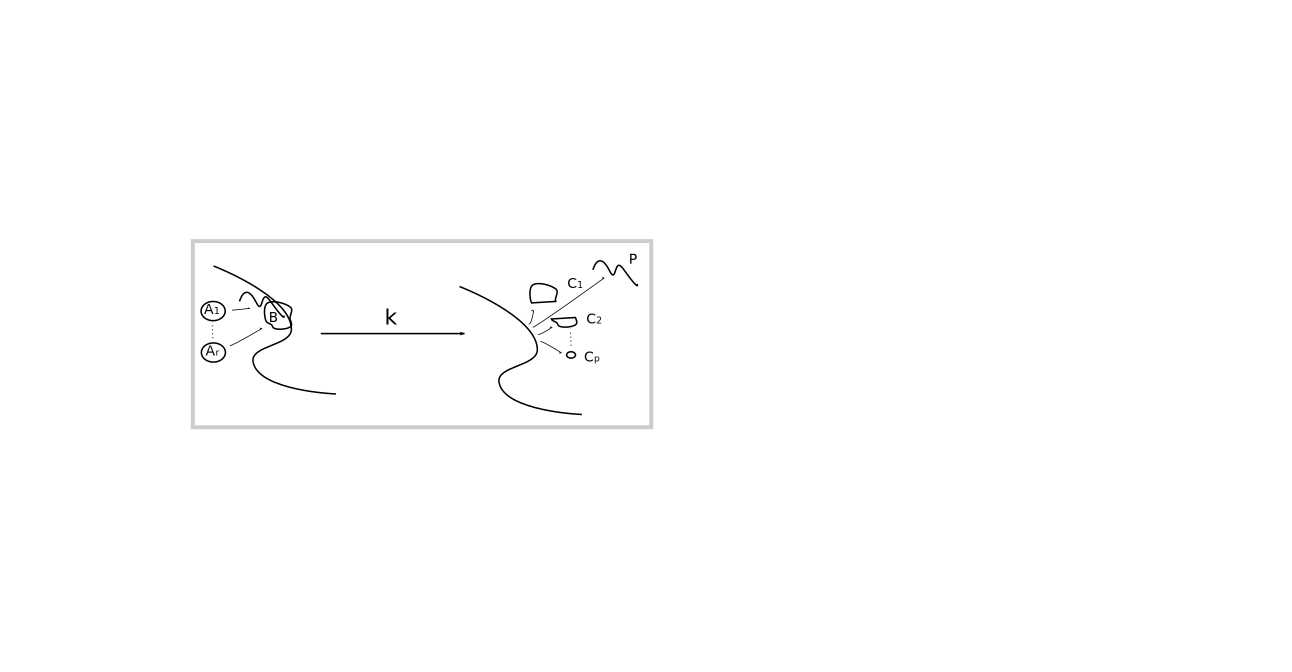
\includegraphics[scale=0.8]{release}
\end{figure}

\paragraph{Input format}
\begin{verbatim}
TransformationTable <name> [<parent_letter> <product_letter>,]^{1..n}
ProductTable <name> <transformation table>
Release <bound chemical> [<chemical> <stoichiometry>]^{0..n} rate <rate> \
  [produces <product table>]
\end{verbatim}

\paragraph{Formula} A \texttt{Release} represents detachment of a bound element from a sequence. An arbitrary number of elements can be used as coreactants to trigger the release, and an arbitrary number of products are released. It is defined by
$$
	\reactionIrr{B + a_1 A_1 + ... + a_r A_r}{\delta_PP + c_1 C_1 + ... + c_p C_p }{k}{}
$$
where
\begin{itemize}
	\item $B$ is of type \texttt{BoundChemical}.
	\item $P$ is of type \texttt{ChemicalSequence}. It is a product that is released if $B$ is a polymerase. In the latter case $\delta_P = 1$ else $\delta_P = 0$.
	\item $A_i$ are of type \texttt{FreeChemical}.
	\item $C_i$ are of type \texttt{FreeChemical}.
	\item $a_i$ and $c_i$ are stoichiometric coefficient.
	\item $k$ is a rate constant.
\end{itemize}

\paragraph{Action} When the reaction is performed, a random $B$ is chosen and removed from the pool (and detached from its sequence). The $A_i$ and $C_i$ pool are changed according to their stoichiometric coefficients. If a \texttt{ProductTable} is defined, it means that the released chemical is a polymerase. A product (a chemical sequence) corresponding to the bound chemical's binding and release points is added. The \texttt{ProductTable} is populated by the second input format of \texttt{ChemicalSequence}.

\paragraph{Rate} The rate is given by
$$
	\lambda = k[B]\prod\limits_{i=1}^{r}[A_i]^{a_i}
$$

\subsubsection{Degradation}

\begin{figure}[!ht]
	\centering
	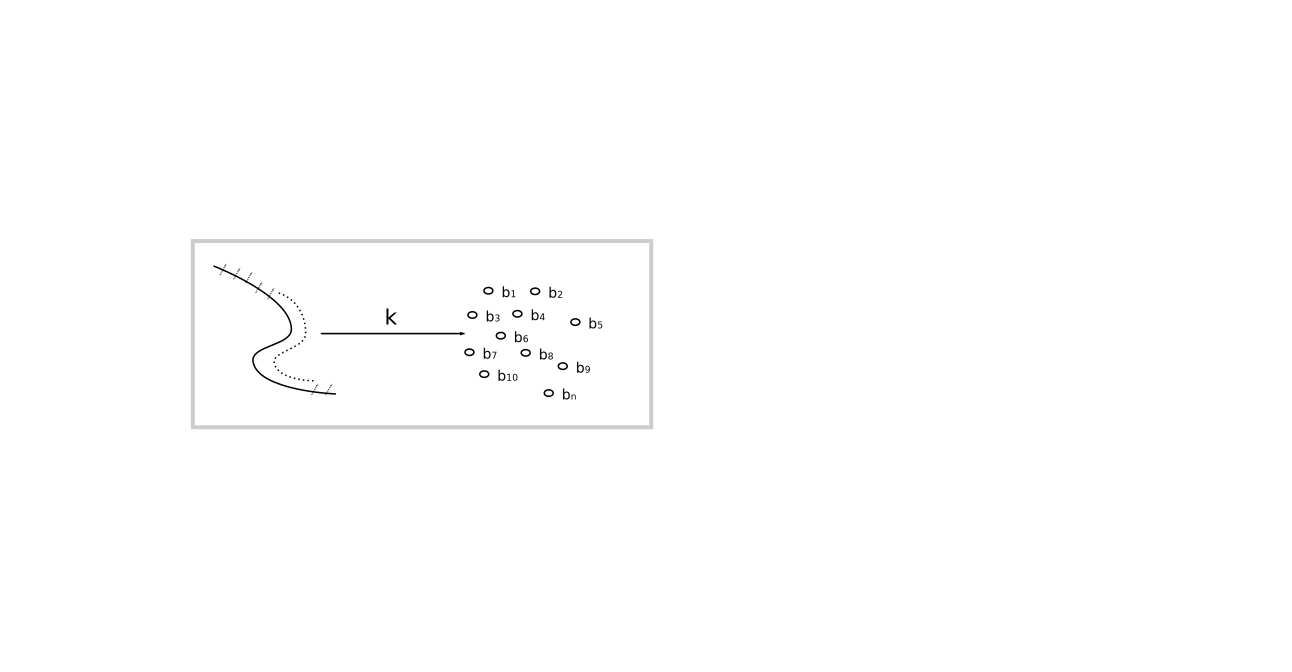
\includegraphics[scale=0.8]{degradation}
\end{figure}

\paragraph{Input format}
\begin{verbatim}
CompositionTable <name> [<letter> [<chemical composing letter>]^{1..m}]^{1..n}
Degradation <chemical sequence> <composition table> <rate>	
\end{verbatim}

\paragraph{Formula} A \texttt{Degradation} represents decomposition of a sequence into base components. It is defined by
$$
	\reactionIrr{CS}{b_1 + b_2 + ... + b_N}{k}{}
$$
where
\begin{itemize}
	\item $CS$ is of type \texttt{ChemicalSequence}.
	\item $b_i$ are of type \texttt{FreeChemical}. They are found in a \texttt{CompositionTable} specified in the reaction.
	\item $k$ is the degradation constant.
\end{itemize}

\paragraph{Action} When the reaction is performed, a $CS$ is removed from the pool. A \texttt{CompositionTable} is specified along the reaction. It allows base-by-base conversion of the sequence of $CS$ into components yielded by degradation. The pools of base components is updated accordingly. In the simulator, a degradation reaction is effectively implemented as a \texttt{ChemicalReaction}.

\paragraph{Rate} The rate is given by
$$
	\lambda = k [CS]
$$

\subsection{Event hierarchy}

\subsection{Rate container hierarchy}

\subsection{Solver hierarchy}


